\documentclass[conference]{IEEEtran}
\IEEEoverridecommandlockouts
% The preceding line is only needed to identify funding in the first footnote. If that is unneeded, please comment it out.
\usepackage{algorithm}
\usepackage{graphicx}
\usepackage{textcomp}
\usepackage{xcolor}
\usepackage{cases, algcompatible, bm, multirow}
\usepackage{pifont}
\usepackage{booktabs}
\usepackage{xspace}
\usepackage{subfigure}
\usepackage{multirow}
\usepackage{threeparttable}

\usepackage{siunitx}
\usepackage{todonotes}  % 启用\todo命令
\usepackage{microtype}  % microtype 包可以微调字符间距，减少断词需求，使排版更紧凑美观
\usepackage{ragged2e}   % 在摘要环境中启用两端对齐
\justifying             % 在摘要环境中启用两端对齐

\usepackage{float}  % 导言区添加
\usepackage{afterpage}
\usepackage{amsmath}  % 数学环境支持

% \usepackage{cite}
% \usepackage{amsmath,amssymb,amsfonts}
% \usepackage{algorithmic}
% \usepackage{graphicx}
% \usepackage{textcomp}
% \usepackage{xcolor}
\def\BibTeX{{\rm B\kern-.05em{\sc i\kern-.025em b}\kern-.08em
    T\kern-.1667em\lower.7ex\hbox{E}\kern-.125emX}}
\begin{document}

\title{RouterAcc: FPGA Acceleration for VLSI Detailed Router via Hierarchical Storage Mapping\\
% {\footnotesize \textsuperscript{*}Note: Sub-titles are not captured in Xplore and
% should not be used}
% \thanks{Identify applicable funding agency here. If none, delete this.}
}

% \author{\IEEEauthorblockN{1\textsuperscript{st} Given Name Surname}
% \IEEEauthorblockA{\textit{dept. name of organization (of Aff.)} \\
% \textit{name of organization (of Aff.)}\\
% City, Country \\
% email address or ORCID}
% \and
% \IEEEauthorblockN{2\textsuperscript{nd} Given Name Surname}
% \IEEEauthorblockA{\textit{dept. name of organization (of Aff.)} \\
% \textit{name of organization (of Aff.)}\\
% City, Country \\
% email address or ORCID}
% \and
% \IEEEauthorblockN{3\textsuperscript{rd} Given Name Surname}
% \IEEEauthorblockA{\textit{dept. name of organization (of Aff.)} \\
% \textit{name of organization (of Aff.)}\\
% City, Country \\
% email address or ORCID}
% \and
% \IEEEauthorblockN{4\textsuperscript{th} Given Name Surname}
% \IEEEauthorblockA{\textit{dept. name of organization (of Aff.)} \\
% \textit{name of organization (of Aff.)}\\
% City, Country \\
% email address or ORCID}
% \and
% \IEEEauthorblockN{5\textsuperscript{th} Given Name Surname}
% \IEEEauthorblockA{\textit{dept. name of organization (of Aff.)} \\
% \textit{name of organization (of Aff.)}\\
% City, Country \\
% email address or ORCID}
% \and
% \IEEEauthorblockN{6\textsuperscript{th} Given Name Surname}
% \IEEEauthorblockA{\textit{dept. name of organization (of Aff.)} \\
% \textit{name of organization (of Aff.)}\\
% City, Country \\
% email address or ORCID}
% }

\maketitle

\begin{abstract}
The semiconductor industry keeps seeking for reducing the design time and efforts in modern integrated circuit implementation, 
while detailed routing is a dead-or-alive critical element in design automation tooling for advanced node enablement, 
which is known as the most time-consuming step in the back-end design flow due to its high complexity and enormous solution space for the very large-scale integration (VLSI) routing problem.

In this paper, we propose a FPGA-based implementation to accelerate the detailed routers, uses efficient memory access management and parallelism to achieve better performance.
Experimental results demonstrate that detailed routers obtain stable and effective acceleration on FPGA. 
Our design gets 2.1$\times$-2.3$\times$, 2.1$\times$-2.5$\times$, 1.3$\times$ speedup compared to TritonRoute, Dr.CU,and current optimum routing kernel acceleration work, 
also obtains 20\% speedup for  detailed routing flow, and 1.0$\times$-1.2$\times$ resource utilization compared to TritonRoute.
\end{abstract}

\begin{IEEEkeywords}
Reconfigurable Computing, FPGA Acceleration, VLSI, Detailed Router
\end{IEEEkeywords}

% \section{Introduction}
% This document is a model and instructions for \LaTeX.
% Please observe the conference page limits. 
%%%%%%%%%%%%%%%%%%%%%%%%%%%%%%%%%%%%%%%%%%%%%%%%%%%%%%%%%%%%%%%%%%%%%%%%%%%%%%%%%%%%%%%%%%%%%%%%%%%%%%%%%
\section{Introduction}
Routing is known as the most complex and time-consuming stage in the physical design flow 
due to its high complexity and enormous solution space for the very large-scale integration (VLSI) routing problem. 
Routing is categorized into global routing and detailed routing. Global routing provides rough guidance with congestion and timing. 
Detailed routing generates exact rectilinear wiring interconnects based on global routing results and 
reduces the design rule violations to satisfy the manufacturability requirements. 
Detailed routing is the primary time bottleneck compared to global routing 
due to strict DRC adherence, larger search space, dynamic data management, manufacturing variability handling, and toolchain interoperability issues.

Detailed routers like TritonRoute\cite{Tr2021} and Dr.CU 2.0\cite{Dr2019} have demonstrated promising performance on industrial benchmarks from ISPD 2018/2019 contests,
are widely accepted in industry and academia to date. 
TritonRoute, as the CPU-driven routing engine within the state-of-the-art open-source RTL-to-GDSII flow, delivers design-rule-clean routing solutions for advanced technology nodes at 16nm and below. 
While this methodology demonstrates robust capability in resolving complex multi-constrained routing problems with high solution quality, 
its inherent computational inefficiency presents a significant bottleneck that markedly impacts turnaround time.

To accelerate routing, existing approaches primarily focus on utilizing partition-based multithreaded CPUs or GPU-accelerated architectures. 
However, these methods exhibit diminishing returns as thread counts increase beyond saturation points, often resulting in measurable quality degradation. 
By customizability of field-programmable gate array (FPGA), the realization of hardware and software co-acceleration with FPGA 
has already achieved competitive performance in accelerating computation tasks in fields like machine learning and scientific computing. 
Similarly, we can benefit from FPGA acceleration in the back-end algorithms 
by customizing and optimizing specific algorithms and detailed routing flow to provide higher performance and faster speed.

In this work, we propose RouterAcc, a highly parallel iterative FPGA acceleration framework 
integrated with multidimensional hierarchical storage mapping for Detailed Router. 
The key contributions are summarized as follows:

\begin{itemize}
    \item A memory access management-enabled FPGA acceleration for detailed router is proposed.Instantiate multiple ram groups to store node information on the corresponding dimension, and Provides a flexible dimension partition architecture, RAM storage can be divided according to specific data characteristics according to X, Y, Z dimensions to maximize resource utilization.
    \item We propose efficient FPGA implementations of detailed routing Kernel on FPGA, and implement detailed routing methods based on grid and A* in workers.
    \item We demonstrate 2.1$\times$-2.3$\times$ speedup in detailed routing without quality degradation of the entire flow over multi-threaded FPGA kernels implementations.More specifically,search operations are independent of each other so that the framework maintains nearly linear scalability with industrial designs.
    \item Through the trial of TritonRoute and Dr.CU accelerating, it is proved that the proposed optimization method has universal significance in the detailed routing scheme, and can be transferred to other similar work besides the example studied in this paper.
\end{itemize}


%%%%%%%%%%%%%%%%%%%%%%%%%%%%%%%%%%%%%%%%%%%%%%%%%%%%%%%%%%%%%%%%%%%%%%%%%%%%%%%%%%%%%%%%%%%%%%%%%%%%%%%%%%
\section{Preliminaries}
\subsection{Detailed Routing Acceleration}

Routing is a complex and critical stage in the physical design of Very Large Scale Integration(VLSI), directly impacting chip performance, power consumption, and manufacturing costs. 
The detailed routing algorithm is critical to routing closure. It generates exact rectilinear wiring interconnects based on global routing results and reduces the design rule violations to satisfy the manufacturability requirements.

In the previous work, BonnRoute\cite{Bo2013} and RegularRoute\cite{Re2013} have made some breakthroughs in reducing wire lengths/through holes and ensuring design compliance through global resource optimization and rule-based hierarchical routing strategies. 
Triggered by the ISPD'18\cite{IS2018} and ISPD'19\cite{IS2019} detailed routing contest, many novel routing methodologies have emerged. 
Kahng et al.\cite{Tr2018}partitioned each layer into parallel panels and formulated the routing problem on each panel as an integer linear program. 
Dr. CU\cite{De2019} proposed an optimal path searching algorithm for minimum-area constraints. Based on this, Li et al. proposed Dr. CU 2.0\cite{Dr2019}to improve the routing quality. 
TritonRoute\cite{Tr2021} employs the rip-up and reroute (RRR) scheme to optimize routing quality and use a routing kernel to find the path of each net. 
Among these algorithms, TritonRoute has the best solution quality and the lowest level of design rule violations (DRCs). 
However, repeated operations on large-scale nets consume most of the total runtime by the routing kernel, establishing it as the dominant efficiency bottleneck in detailed routing flows.

To address the critical challenge of time-consuming routing processes in routing flow, researchers have explored heterogeneous acceleration platforms. 
For path planning acceleration using the A* algorithm, Zhou et al.\cite{FP2020} demonstrated 37-75$\times$ acceleration via 8-port cache and array-based OPEN lists. 
Osama et al.\cite{Fa2021} developed an FPGA implementation with 50-100$\times$ speedup through 8-way parallel evaluators and cache-optimized memory access. 
However, none of these methods have been applied to the detailed routing kernel.
For maze routing acceleration, Lin et al.\cite{GA2023} proposed GAMER 
that achieved 16$\times$ acceleration for coarsened maze routing through sweeping-style parallelism. 
Jiang et al.\cite{FP2022} implemented an FPGA-based batched maze routing kernel, achieving 3.1$\times$ speedup over CPU implementations with <1\% wirelength degradation. 
However, the performance of these methods on detailed routing is constrained by data dependencies and memory management.

\subsection{Memory Access Bottleneck of Detailed Routing}

The core of detailed routing algorithms lies in the highly efficient heuristic path-planning method, like the A* search algorithm. 
However, the existing optimizations on the A* algorithm are mainly aimed at computational optimization, 
and the bottleneck in maintaining the open list and the closed list is outstanding, especially when performing many iterative operations. 

Zhou et al.\cite{FP2020} found that when the A* algorithm runs in a single thread, the operations of the open list consume 95\% of the total time. 
After distributing the software process into eight threads, the open list operations still consume 88\% of total time. 
Thus the architecture does not solve the problem of time-consuming memory access, and suffers from inefficient resource utilization when processing high-obstacle density maps and frequent cache misses degrade performance predictability. 
Therefore, the most time-consuming open list and close list operations have become the bottleneck of A* algorithm acceleration. 
The accelerated A* techniques exhibit broad applicability across various path-searching implementations. 
Given the fundamental similarities in routing paradigms, particularly in maze routing algorithms and heuristic flow implementation methodologies, 
these acceleration strategies demonstrate significant transfer potential beyond the specific use cases examined in this study. 



% The core of routing algorithms lies in the highly efficient heuristic path-planning method, like the A-star (or A$\ast$ ) search algorithm.  
% However, the existing optimizations on the A* algorithm are mainly aimed at computational optimization, and the bottleneck in 
% maintaining the open list and a closed list is obviously outstanding, especially when performing many iterative operations.  
% For the typical path planning method (A*)acceleration by using FPGA, Zhou et al.[7] demonstrated 37-751$\times$ acceleration via 8-port cache 
% and array-based OPEN lists, but the architecture suffers from inefficient resource utilization when processing high-obstacle density maps,
% where frequent cache misses degrade performance predictability. 

\begin{figure}[htbp]
    \centering
    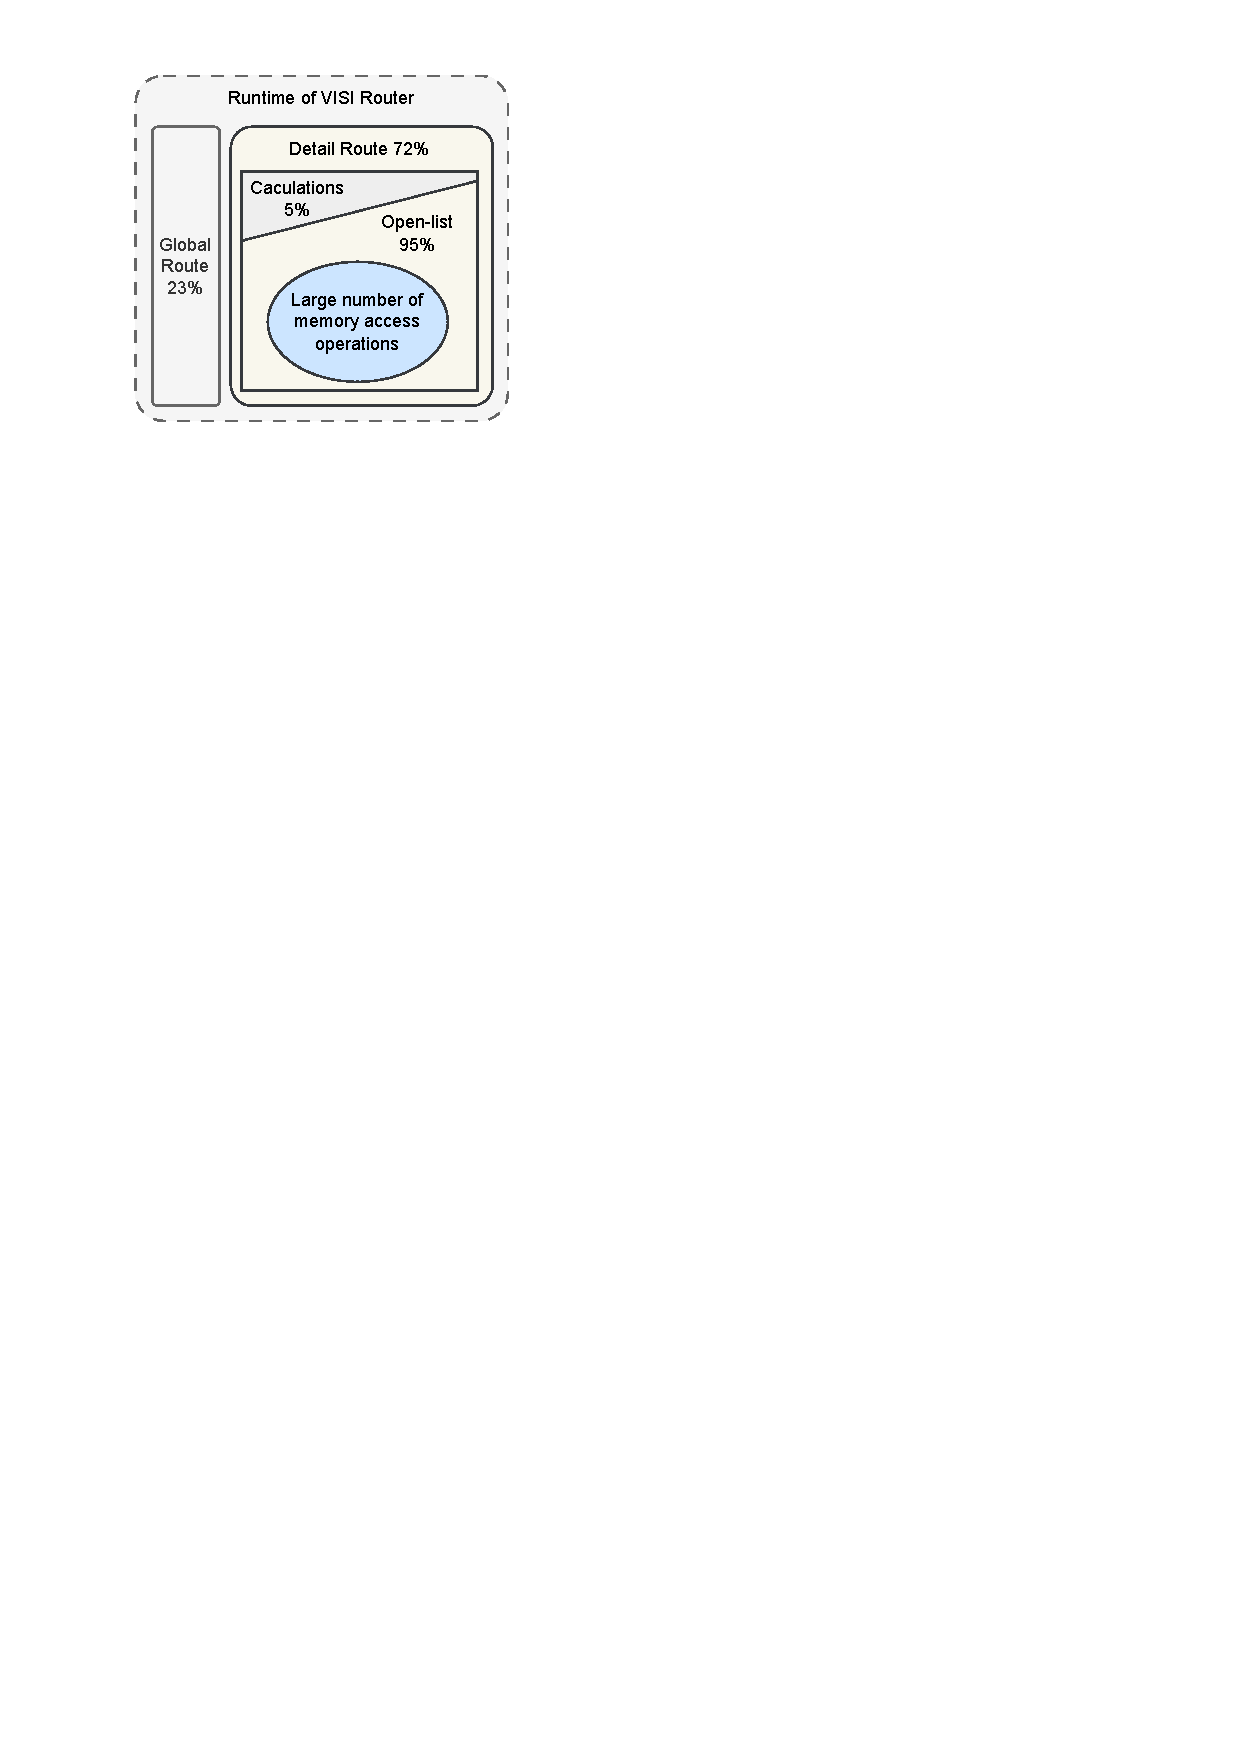
\includegraphics[width=7cm]{figures/Execution Time.pdf}
    \caption{Detailed routing takes up most time in the routing process, and most of it is memory access time.}
    \label{fig:Execution Time} % 标签紧跟标题
\end{figure}

Osama et al.[8] developed an FPGA implementation with 50-1001$\times$ speedup through 8-way parallel evaluators and cache-optimized memory access. 
Nevertheless, its fixed 256$\times$256 grid mapping and complex 5$\times$5 caching mechanism restrict scalability for large-scale scenarios. 
Jiang et al.[9] implemented an FPGA-based batched maze routing kernel achieving 3.11$\times$ speedup over CPU implementations with < 1\% 
wirelength degradation, but its performance is constrained by data dependency management and limited scalability when handling heterogeneous net sizes. 
Meanwhile, Lin et al.[10] proposed GAMER, a GPU-accelerated maze routing scheme that achieved 161$\times$ acceleration for coarsened maze routing through sweeping-style parallelism. 
However, its performance gain diminishes in fine-grained routing stages, and the qualitydriven batch partitioning strategy introduces 
additional scheduling overhead that limits throughput. 

\subsection{Versatility and Scalability}
The above proposed acceleration methodology for detailed routing preserves the quality of the entire implementation flow for 
multithreaded FPGA core architectures. Actually, the accelerated A* techniques exhibit broad applicability across various path-searching 
implementations. Given the fundamental similarities in routing paradigms,  particularly in maze routing algorithms and heuristic flow implementation 
methodologies, these acceleration strategies demonstrate significant transfer potential beyond the specific use cases examined in this study. 





%%%%%%%%%%%%%%%%%%%%%%%%%%%%%%%%%%%%%%%%%%%%%%%%%%%%%%%%%%%%%%%%%%%%%%%%%%%%%%%%%%%%%%%%%%%%%%%%%%%%%%%%%%%%%
\section{Algorthm}
\subsection{Detailed Routing Algorthm Analysis}
Conventional framework of detailed routing algorithm we employ follows a structured flow, as illustrated in Algorithm 1. 
Given the global routing results of the benchmarks (e.g..def and.guides files), we perform a track assignment step following the method described in [11], aligning all nets to predefined routing tracks. 
This preprocessing phase extracts and constructs essential data structures, such as routing grids, net objects, and guide constraints, which serve as inputs to the detailed routing engine. 
The ultimate goal is to produce a DRC-clean routing result with full connectivity, starting from these coarse global routing guides.

%%eg [11]M.-P. Wong, W.-H. Liu, and T.-C. Wang, “Negotiation-based track assignment considering local nets,” in Proc. 21st Asia South Pac. Design Automat. Conf. (ASP-DAC), Macau, China, 2016, pp. 378–383.

\begin{algorithm}[hpt]
\caption{Detailed Routing Flow}
\label{alg:detail_routing_algorithm}
\begin{algorithmic}[1]
\Statex \textbf{Input:} base-data structure, global routing guides
\Statex \textbf{Output:} full connected nets
\STATE \text{InitDb()}, \text{InitPreRouteNet()}

\WHILE{$iter < maxIter$}
    \STATE \text {$drcNets \gets [net_{i}: while$ $ net_{i} \in Nets,$$if$ $net_{i}.drcScore \neq 0]$}
    \WHILE{$\text{$net$} \in \text{$drcNets$}$}
        \STATE $\text{$ucPins$} \gets \text{$GetPins(net)$}$
        \WHILE {$ucPins \neq \emptyset$}
            \STATE $\text{$tpin$} \gets \mathop{\arg\max}\limits_{pin \in ucPins} \text{$pin.cost$}$
            \STATE $\text{$cPins$} \gets \text{$cPins$} \cup \text{$tPin$}$, $\text{$ucPins$} \gets \text{$ucPins$} \setminus \text{$tPin$}$
            \STATE $\text{$sPin$} \gets \text{GetNextPin(\text{$ucPins$})}$
            \STATE \text{FPGA-OptimizedRoutingKernel($sPin$,$cPins$)}
        \ENDWHILE
    \ENDWHILE
    
    \STATE \text{UpdateDRC()}, \text{UpdateNets()}
\ENDWHILE
\STATE \text{UpdateDb()}
\end{algorithmic}
\end{algorithm}


The detailed routing flow, as depicted in Algorithm 1, comprises multiple sequential phases. Initially, the design database is initialized via InitDb(), and essential nets are pre-routed using InitPreRouteNet(). Following this, nets are evaluated based on their design rule check scores, and those exhibiting violations are prioritized for further processing.
The outer loop (lines 2 to 14) performs iterative rip-up and reroute operations, bounded by a predefined maximum iteration count. In each iteration, the set of nets with non-zero DRC scores is extracted. For each net in drcNets, the set of unconnected pins is identified (line 5). The algorithm proceeds to incrementally connect these pins by repeatedly selecting the pin with the highest routing cost as the current target, moving it to the connected pin set, and identifying the next nearest source pin (lines 6–9).
Routing between the selected source and target pins uses the Optimized Routing kernel, which leverages high-throughput hardware acceleration. This process continues until all pins in the net are connected. After net-level rerouting, the global DRC state and net data structures are updated accordingly . Upon convergence or exhaustion of iterations, a final database update is performed, reflecting the complete routing solution.


\begin{algorithm}[hpt]
    \caption{FPGA-Optimized Routing Kernel Algorithm}
    \label{alg:FPGA in A* algorithm}
    \begin{algorithmic}[1]
    \Statex \textbf{Input:} source pin $s$, target pins $\{t_1, \dots, t_n\}$
    \Statex \textbf{Output:} minimum-cost routing paths
    \Statex \textbf{Prepare:} priority queue $Q$, cost map $T$, flag map $F$, graph batch $G$ $\{G_1, ..., G_N\}$, direction set $D$ $\{E, W, N, S, U, D\}$ in BRAM
    
    \STATE Initialize $N$ grid maps in BRAM
    \FOR {$G_k \in G$ \textbf{in parallel}}
        \State \textbf{set} $Q^{(k)}$, $T^{(k)}(v) \gets \infty$, $F^{(k)}(v) \gets 0, \forall v$; $T^{(k)}(s) \gets 0$
        \WHILE{$Q^{(k)} \neq \emptyset$ }
            \STATE $v \gets \text{MinCost($Q^{(k)}$)}$
            \STATE $if$ $v \in \{t_1,...,t_n\}$ \textbf{break}
            \FOR{$u \in D $ \textbf{in parallel}}
                \State $c \gets T^{(k)}(v) + \Delta(v,u)$
                \IF{$c < T^{(k)}(u)$}
                    \State $T^{(k)}(u) \gets c$, $F^{(k)}(u) \gets 1$, $u.parent \gets v$
                    \State \text{Update($Q^{(k)}$)}
                \ENDIF
            \ENDFOR
        \ENDWHILE
    
        \State \text{BackTrack Path}
    \ENDFOR
\end{algorithmic}
\end{algorithm}


% % \clearpage  % 结束当前页
% % \vspace*{0pt}  % 避免覆盖已有内容
% \afterpage{  % 当前页结束后执行
\begin{figure*}[!ht]
    \centering
    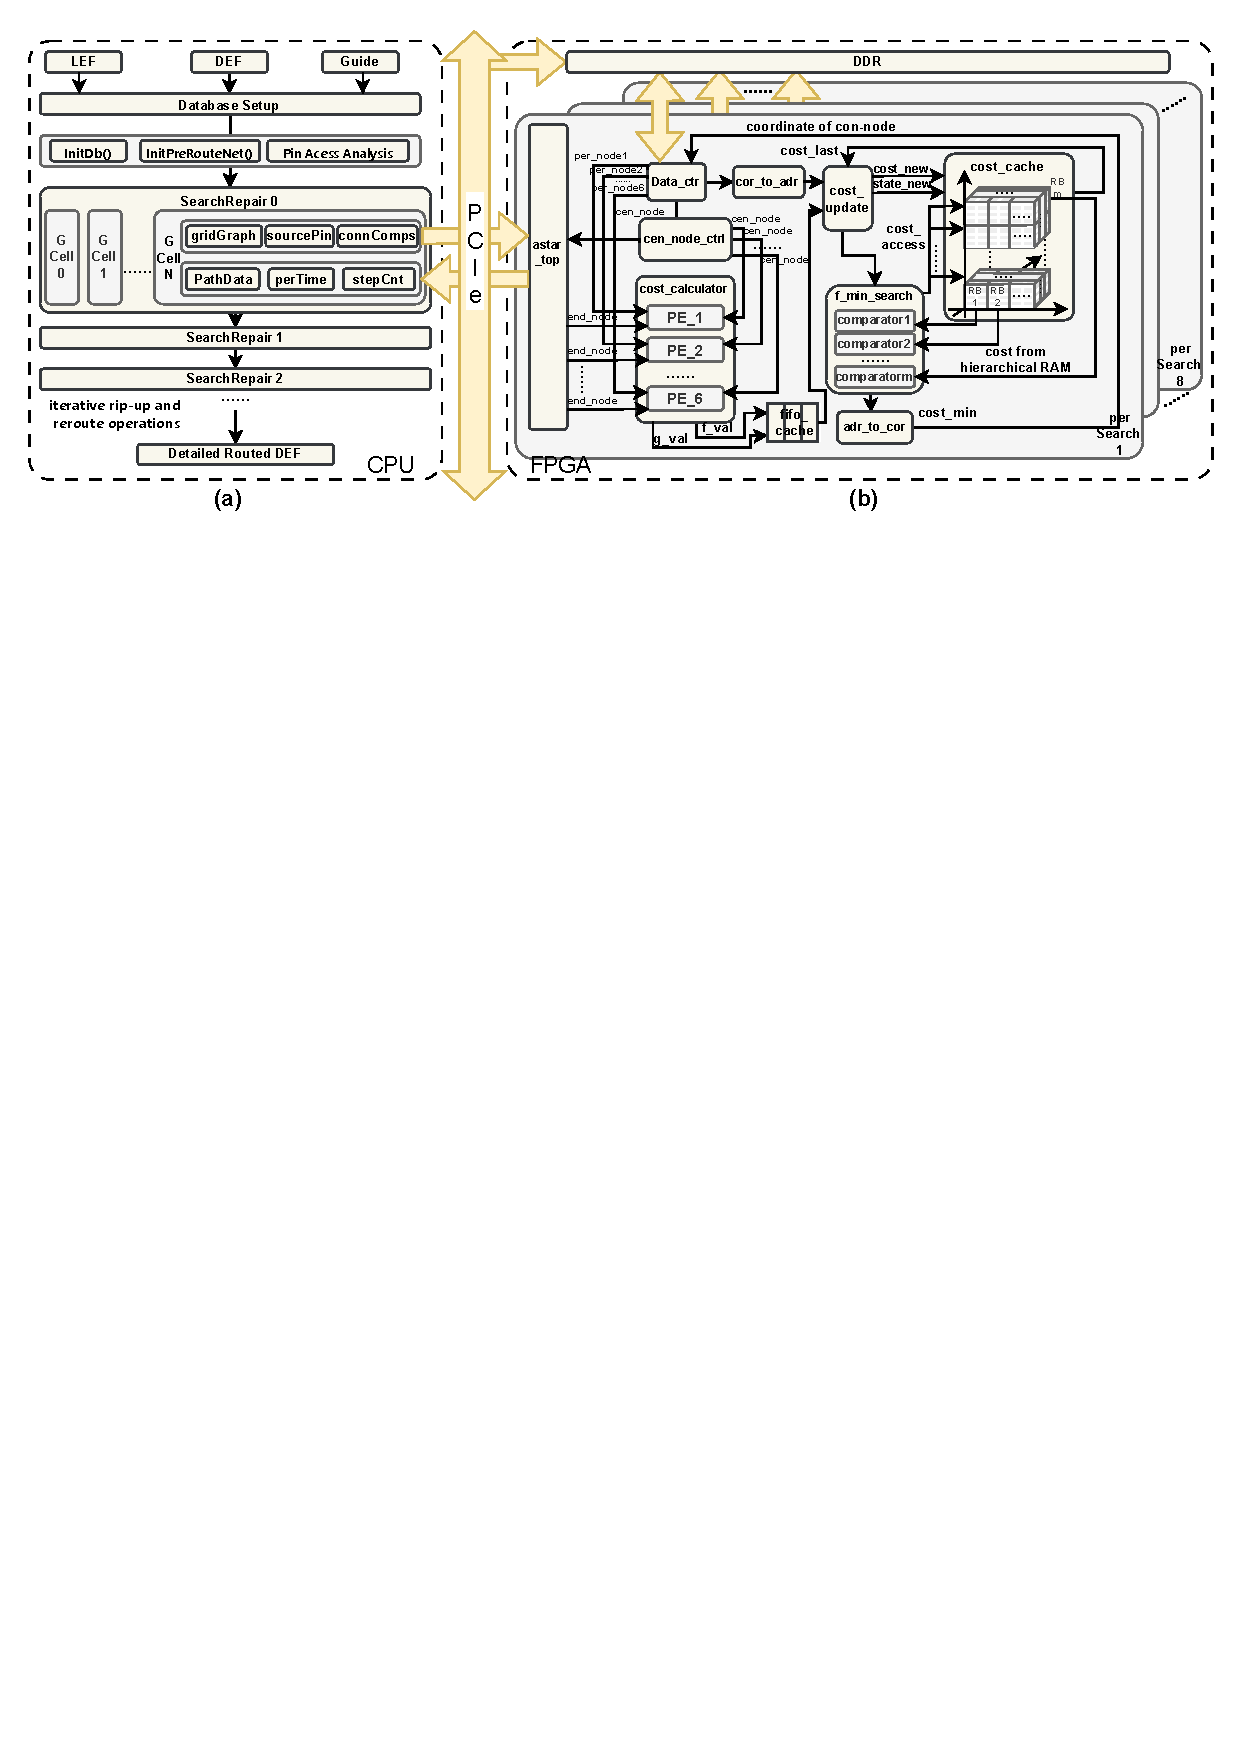
\includegraphics[width=\textwidth]{figures/Arch Overview.pdf}
    \caption{The overview structure.(a) The flow of detailed router on GPU.(b) The overview of FPGA acceleration framework.}
    \label{fig:overview} % 标签紧跟标题
\end{figure*}
% }

\subsection{Routing Kernel and Generating Routing Graphs Algorthm Analysis}
The most popular detailed routing methods, like TritonRoute[?] and Dr. CU[?], are both executed by the maze routing kernel to connect all pins on the nets with minimal cost. 
In the actual computing stage, the nets will first abstracted as grid graphs. Each pin pn is equivalent to a set of vertices Sn located on its position, 
then utilize the priority queue and some heuristic methods to improve the quality and speed.Taking TritonRoute[?] as an example, it uses A* (A-STAR) algorithm to explore the route and sets weight for each node.
The weight is a heuristic function f (x) : f (x) = g(x) + h(x), where the function g(x) is the distance or cost from the starting node to current state x, and the function h(x) defines the estimated distance or cost from current state x to the end node. 
We call the function value of f (x) the f value. 

In each round of A* search, we extract the state with the minimum f value from the open list, expand its outer neighbors and check for duplication.
In general, Batched maze routing kernel is executed on a large batch of graphs in the detailed routing stage. There are almost 1,000 ~ 10,000 graphs (nets) in one batch without data dependency between any two graphs, providing a powerful condition for parallelization operation on FPGA to achieve efficient acceleration.

However, the typical maze routing algorithm should be modified to adapt the property of FPGA,as Algorithm 2 shows.
The grid map is initialized in the memory and the start and end nodes are sent to the design so it can start solving the map.
The priority queue Q, the temporary cost set T, and the vertices' state set F used in the hardware-optimized maze routing algorithm are also implemented on hardware.
At the outer level, multiple routing graphs are processed concurrently, exploiting batch-level parallelism with thousands of nets in BRAM.
At the inner level, for each graph, neighbour expansions across multiple directions are executed in parallel to accelerate wavefront propagation.
This fine-grained directional parallelism, combined with hardware-managed cost updates and queue operations, enhances routing throughput on FPGA.

In the process of generating routing diagram, take TritonRoute[?] as an example, through the breadth-first search (BFS) path planning method of extending and updating wavefront, 
the wavefront is dynamically generated and explored in six directions, southeast, northwest and upper, lower, and lower, to gradually update the cost information of each node to realize the path between the target point and the starting point.
It can also be deployed on FPGAs for acceleration through full parallelism and data processing optimization.
%%%%%%%%%%%%%%%%%%%%%%%%%%%%%%%%%%%%%%%%%%%%%%%%%%%%%%%%%%%%%%%%%%%%%%%%%%%%%%%%%%%%%%%%%%%%%%%%%%%%%%%%%%%%%%%%%%%%%%%%%%%%%%%%%%%%%%%%%%%%%%%%%%%%%%
\section{Design of Acceleration Module}
\subsection{The Overview of FPGA Acceleration Framework}
Conventional implementations of A* search usually use two lists to store the states during its expansion, i.e., the \textbf{open list} and the \textbf{closed list}. 
The closed list stores all the visited states, and is used to prevent unnecessary repeated expansion of the same state. This list is often implemented by a linked hash table to detect the duplicated nodes. 
The open list normally stores the states whose successors have not been fully explored yet. The open list uses a priority queue as its data structure, typically implemented by a binary heap. 
States in the open list are sorted according to the function value of heuristic function f (x).

A lot of work proves that memory access is the time bottleneck of the algorithm compared to the computation time, as Figure~\ref{fig:Execution Time} shows.
So our work is dedicated to propose a FPGA-based implementation to accelerate the detailed routers, uses efficient memory access management and parallelism to achieve better performance.
Figure~\ref{fig:overview} shows the overview of FPGA acceleration framework.

\begin{figure*}[!ht]
    \centering
    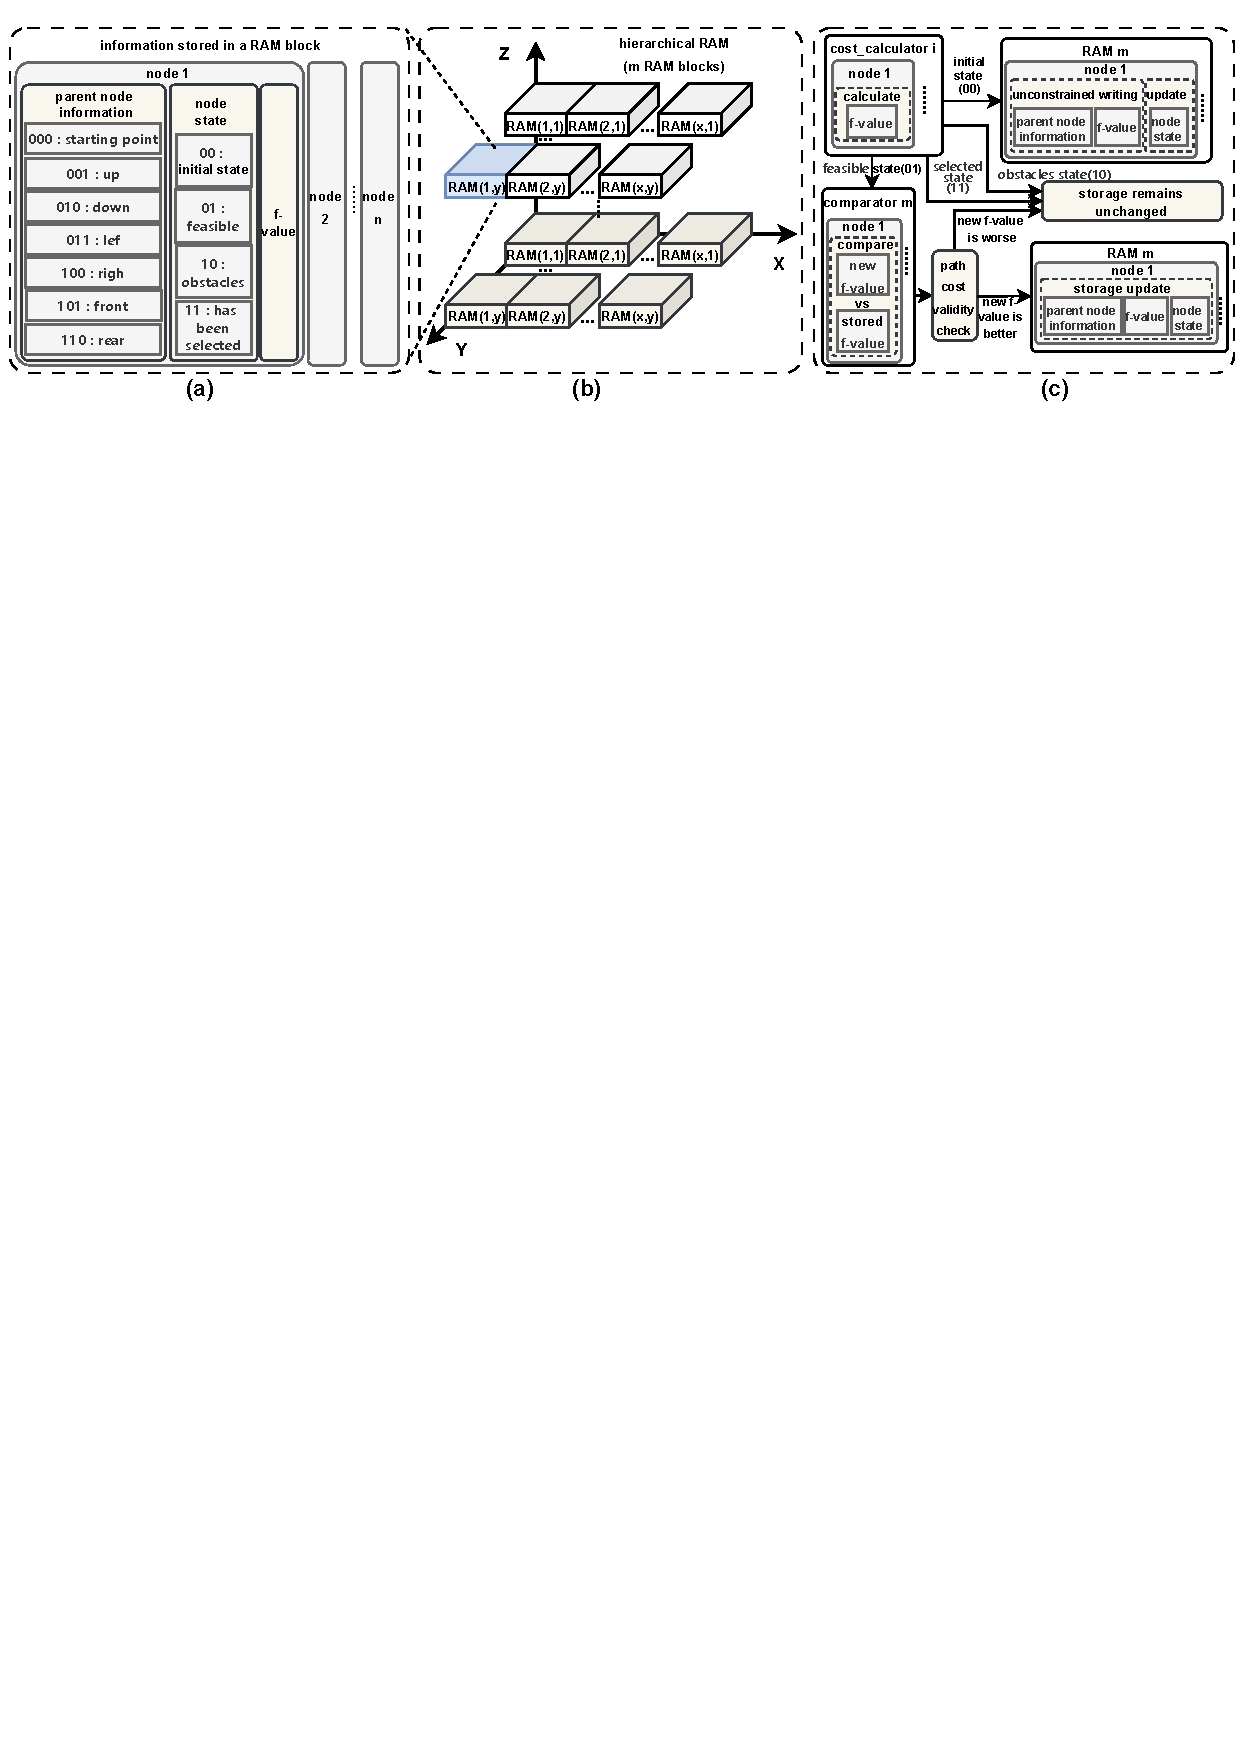
\includegraphics[width=\textwidth]{figures/RAM Data.pdf}
    \caption{RAM data structure on FPGA.(a)Information stored in a RAM block .(b)hierarchical RAM(a total of n RAM blocks).(c)The f-value update logic.}
\end{figure*}


\subsection{Hierarchica RAM Blocks}
Instantiate multiple ram groups to store node information on the corresponding dimension.
Traditional FPGA-based path planning algorithms have significant bottlenecks in maintaining \textbf{open list} and \textbf{closed list}.
The dynamic sorting mechanism requires the storage structure to be reordered after each search iteration. This frequent sorting operation will not only consume a lot of programmable logic resources, but also produce a processing delay that does not match the hardware architecture, which seriously restricts the real-time performance of the system.
In addition, dynamic memory management of variable-length data structures leads to fragmented access to Block RAM, resulting in reduced hardware resource utilization.

To solve this problem we observed, the dimensional organization of RAM can be efficiently managed through hierarchical mapping, in FPGA-based storage architecture design, as fig1 shows.
For 2D data structure, row-priority storage strategy can be adopted, so that each RAM module can store the data node corresponding to the row (first dimension) independently.
When extended to a three-dimensional structure, each RAM module can be responsible for storing node information in a fixed plane, such as the third dimension.
Through the introduction of address mapping module, high-dimensional addresses (such as three-dimensional coordinates (x,y,z)) can be converted into two-dimensional storage addresses inside each RAM module. This hierarchical mapping mechanism significantly improves storage access efficiency and data throughput.

In addition, we offer a flexible dimension division architecture. The RAM storage can be divided into X, Y, and Z dimensions based on specific data characteristics, and can be adjusted according to the actual wiring situation, thereby achieving better acceleration effects.
We initially use simple methods such as the y-z plane for partitioning, but the number of calculation periods is extremely large. This is because shuttling through the y-z plane frequently occurs during wiring. Therefore, we have made the following improvements:
1) Change the RAM division in the y-z plane direction to the x-y direction, and change the shuttle in the y-z plane to x-y to reduce the number of points inside the RAM;
2) Further meshes are carried out within the x-y plane to reduce the jurisdiction area of each RAM and further compress the maximum period of the minimum value search within each RAM.
The above two points can effectively reduce the overall path search time.

By introducing the address mapping module, high-dimensional addresses (such as three-dimensional coordinates (x,y,z)) can be converted into two-dimensional storage addresses within each RAM module. 
This hierarchical mapping mechanism significantly improves the efficiency of storage access and data throughput.
The address mapping logic is as follows:

% \[
\noindent As the known coordinate values is (x,y,z), we define:
\begin{align*}
    X_{\text{BLOCK\_WD}} &: \text{the number of data in x-dimension of RAM} \\
    Y_{\text{BLOCK\_WD}} &: \text{the number of data in y-dimension of RAM} \\
    Z_{\text{BLOCK\_WD}} &: \text{the number of data in z-dimension of RAM}
    \end{align*}
% X_BLOCK_WD:the number of data in the x-dimension of RAM
% Y_BLOCK_WD:The number of data in the y-dimension of RAM
% Z_BLOCK_WD:The number of data in the z-dimension of RAM
\begin{align*}
    x_{\text{f\_ram\_sel\_cnt}} &= \frac{\text{per\_x}}{X_{\text{BLOCK\_WD}}} \\
    y_{\text{f\_ram\_sel\_cnt}} &= \frac{\text{per\_y}}{Y_{\text{BLOCK\_WD}}} \\
    z_{\text{f\_ram\_sel\_cnt}} &= \frac{\text{per\_z}}{Z_{\text{BLOCK\_WD}}}
    \end{align*}
% x_f_ram_sel_cnt=per_x/X_BLOCK_WD
% y_f_ram_sel_cnt=per_y/Y_BLOCK_WD
% z_f_ram_sel_cnt=per_z/Z_BLOCK_WD
The RAM enable signal is:
\begin{align*}
    f_{\text{ram\_sel}} &= x_{\text{f\_ram\_sel\_cnt}} \\
    &\quad + y_{\text{f\_ram\_sel\_cnt}} \times X_{\text{RAM\_NUM}} \\
    &\quad + z_{\text{f\_ram\_sel\_cnt}} \times X_{\text{RAM\_NUM}} \times Y_{\text{RAM\_NUM}}
    \end{align*}
% f_ram_sel=x_f_ram_sel_cnt+y_f_ram_sel_cnt*X_RAM_NUM+z_f_ram_sel_cnt*X_RAM_NUM*Y_RAM_NUM
The address of RAM Blocks on-chip is:
\begin{align*}
     f_{\text{ram\_sel}} &= x_{\text{f\_ram\_sel\_cnt}} \\
     &\quad + y_{\text{f\_ram\_sel\_cnt}} \times X_{\text{RAM\_NUM}} \\
     &\quad + z_{\text{f\_ram\_sel\_cnt}} \times X_{\text{RAM\_NUM}} \times Y_{\text{RAM\_NUM}}
    \end{align*}
% \]

\subsection{Data Structure and Update Control}
After the path cost calculation module completes the f-value generation of the adjacent nodes of the central node, the system executes the storage update process based on logical control.
First, Cost\_cache memory is accessed through the coordinate addressing mechanism to extract the status flag bit and historical f-value of the target node: If the flag bit is detected as the initial state (00), the new f-value and status flag are directly written without constraints;
If the status flag is explored state (01), the hardware comparator is triggered to perform the numerical relationship determination of the new f-value and the stored f-value in parallel, and the path cost validity check is performed at the same time to avoid calculation anomalies.
Finally, the storage unit is selectively updated according to the judgment result: for the initial state node to load new data completely, the explored state node only performs overwrite storage and synchronously updates the state when the new f-value is better.
This mechanism uses the state-driven conditional write strategy to reduce the redundant access to memory and data overwrite operations while maintaining the principle of path planning optimality.

% \begin{figure}[htbp]
%     \centering
%     \includegraphics[width=8cm]{figures/acceleration/Cost Cache.jpg}
%     \caption{Instantiate multiple ram block storage}
% \end{figure}

\begin{figure}[htbp]
    \centering
    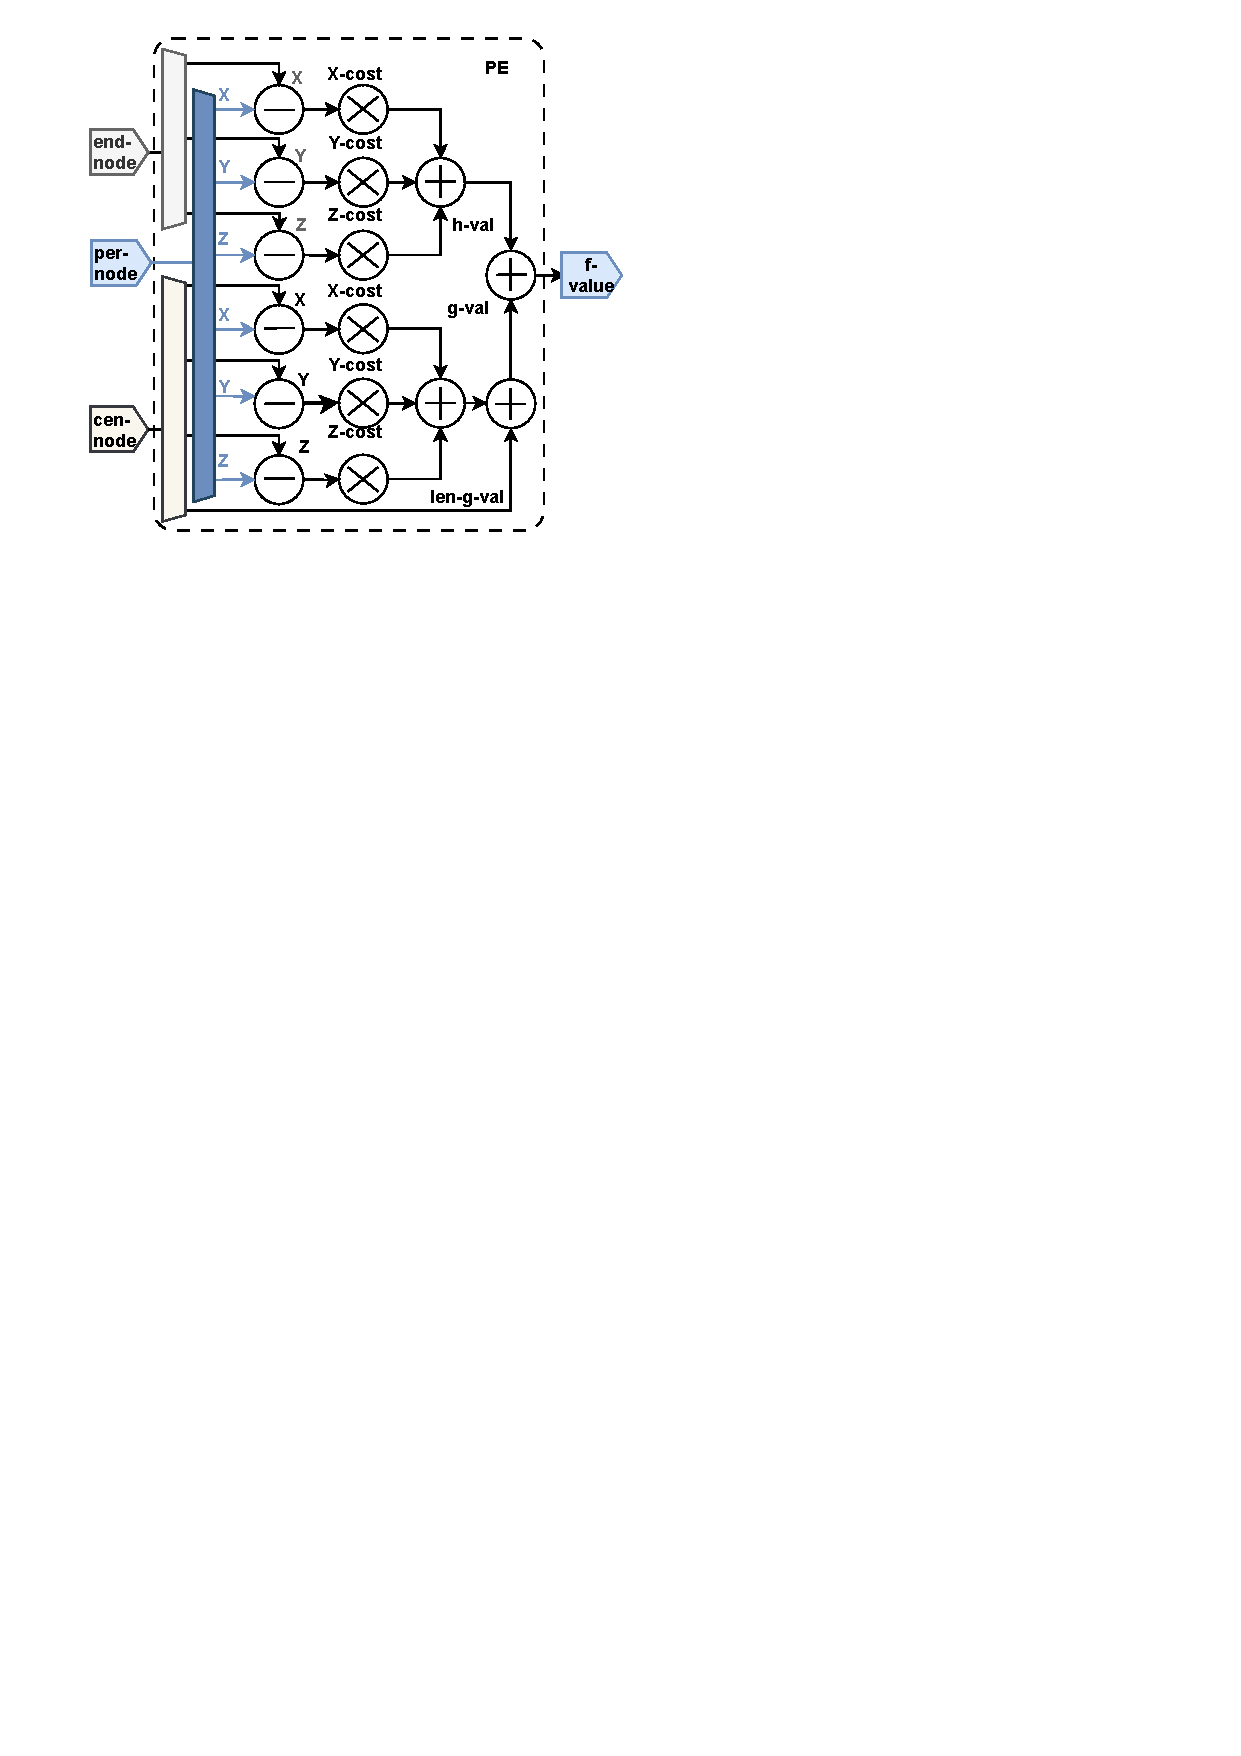
\includegraphics[width=7cm]{figures/PE.pdf}
    \caption{The PE of Cost\_Calculator module.}
\end{figure}

\subsection{Calculate Cost}
\textbf{Cost\_calculator module} calculates the f-values of 6 peripheral points in parallel according to the input center point and surrounding point information.
The information in 6 directions is calculated in parallel to the Manhattan distance, and the F value of the 6 surrounding points is calculated based on F=G+H.

\textbf{Cost\_calculator module} 


\begin{table*}[!htbp]
    \caption{Comparison of performance between TritonRoute [?] Dr.CU [?] and our FPGA acceleration to complete batched maze routing kernel with ISPD 2018 [?] contest benchmarks.}
    \begin{tabular}{|c|llllc|cccllcll|}
    \hline
    \multirow{2}{*}{ispd18} & \multicolumn{5}{c|}{\multirow{2}{*}{ISPD' 18 quality score}}                                                               & \multicolumn{8}{c|}{Routing Kernel(8 kernels)}                                                                                                                                                                                                      \\ \cline{7-14} 
                            & \multicolumn{5}{c|}{}                                                                                                      & \multicolumn{5}{c|}{Runtime(s)}                                                                                                                       & \multicolumn{3}{c|}{Speed-up}                                                               \\ \hline
                            & \multicolumn{1}{c|}{TR} & \multicolumn{1}{c|}{CU} & \multicolumn{1}{c|}{RA-TR} & \multicolumn{1}{l|}{{[}1{]}-CU} & CoRA-TR & \multicolumn{1}{c|}{TR}     & \multicolumn{1}{c|}{CU} & \multicolumn{1}{c|}{RA-TR}   & \multicolumn{1}{l|}{{[}1{]}-CU} & \multicolumn{1}{c|}{CoRA-TR} & \multicolumn{1}{c|}{RA-TR} & \multicolumn{1}{l|}{{[}1{]}-CU} & \multicolumn{1}{c|}{CoRA-TR} \\ \hline
    testl                   & \multicolumn{1}{l|}{}   & \multicolumn{1}{l|}{}   & \multicolumn{1}{l|}{}      & \multicolumn{1}{l|}{}           &         & \multicolumn{1}{c|}{4.41}   & \multicolumn{1}{c|}{}   & \multicolumn{1}{c|}{2.03}    & \multicolumn{1}{l|}{}           & \multicolumn{1}{l|}{}        & \multicolumn{1}{c|}{2.2x}  & \multicolumn{1}{l|}{}           &                              \\ \hline
    test2                   & \multicolumn{1}{l|}{}   & \multicolumn{1}{l|}{}   & \multicolumn{1}{l|}{}      & \multicolumn{1}{l|}{}           &         & \multicolumn{1}{c|}{58.86}  & \multicolumn{1}{c|}{}   & \multicolumn{1}{c|}{25.93}   & \multicolumn{1}{l|}{}           & \multicolumn{1}{l|}{}        & \multicolumn{1}{c|}{2.3x}  & \multicolumn{1}{l|}{}           &                              \\ \hline
    test3                   & \multicolumn{1}{l|}{}   & \multicolumn{1}{l|}{}   & \multicolumn{1}{l|}{}      & \multicolumn{1}{l|}{}           &         & \multicolumn{1}{c|}{110.07} & \multicolumn{1}{c|}{}   & \multicolumn{1}{c|}{52.4}    & \multicolumn{1}{l|}{}           & \multicolumn{1}{l|}{}        & \multicolumn{1}{c|}{2.1x}  & \multicolumn{1}{l|}{}           &                              \\ \hline
    test4                   & \multicolumn{1}{l|}{}   & \multicolumn{1}{l|}{}   & \multicolumn{1}{l|}{}      & \multicolumn{1}{l|}{}           &         & \multicolumn{1}{c|}{244.48} & \multicolumn{1}{c|}{}   & \multicolumn{1}{c|}{211.68}  & \multicolumn{1}{l|}{}           & \multicolumn{1}{l|}{}        & \multicolumn{1}{c|}{2.3x}  & \multicolumn{1}{l|}{}           &                              \\ \hline
    test5                   & \multicolumn{1}{l|}{}   & \multicolumn{1}{l|}{}   & \multicolumn{1}{l|}{}      & \multicolumn{1}{l|}{}           &         & \multicolumn{1}{c|}{109.42} & \multicolumn{1}{c|}{}   & \multicolumn{1}{c|}{40.39}   & \multicolumn{1}{l|}{}           & \multicolumn{1}{l|}{}        & \multicolumn{1}{c|}{2.3x}  & \multicolumn{1}{l|}{}           &                              \\ \hline
    test6                   & \multicolumn{1}{l|}{}   & \multicolumn{1}{l|}{}   & \multicolumn{1}{l|}{}      & \multicolumn{1}{l|}{}           &         & \multicolumn{1}{c|}{165.39} & \multicolumn{1}{c|}{}   & \multicolumn{1}{c|}{77.33}   & \multicolumn{1}{l|}{}           & \multicolumn{1}{l|}{}        & \multicolumn{1}{c|}{2.1x}  & \multicolumn{1}{l|}{}           &                              \\ \hline
    test7                   & \multicolumn{1}{l|}{}   & \multicolumn{1}{l|}{}   & \multicolumn{1}{l|}{}      & \multicolumn{1}{l|}{}           &         & \multicolumn{1}{c|}{246.12} & \multicolumn{1}{c|}{}   & \multicolumn{1}{c|}{111.98}  & \multicolumn{1}{l|}{}           & \multicolumn{1}{l|}{}        & \multicolumn{1}{c|}{2.2x}  & \multicolumn{1}{l|}{}           &                              \\ \hline
    test8                   & \multicolumn{1}{l|}{}   & \multicolumn{1}{l|}{}   & \multicolumn{1}{l|}{}      & \multicolumn{1}{l|}{}           &         & \multicolumn{1}{c|}{256.73} & \multicolumn{1}{c|}{}   & \multicolumn{1}{c|}{125.29}  & \multicolumn{1}{l|}{}           & \multicolumn{1}{l|}{}        & \multicolumn{1}{c|}{2.1x}  & \multicolumn{1}{l|}{}           &                              \\ \hline
    test9                   & \multicolumn{1}{l|}{}   & \multicolumn{1}{l|}{}   & \multicolumn{1}{l|}{}      & \multicolumn{1}{l|}{}           &         & \multicolumn{1}{c|}{264.21} & \multicolumn{1}{c|}{}   & \multicolumn{1}{c|}{128.19}  & \multicolumn{1}{l|}{}           & \multicolumn{1}{l|}{}        & \multicolumn{1}{c|}{2.1x}  & \multicolumn{1}{l|}{}           &                              \\ \hline
    test10                  & \multicolumn{1}{l|}{}   & \multicolumn{1}{l|}{}   & \multicolumn{1}{l|}{}      & \multicolumn{1}{l|}{}           &         & \multicolumn{1}{c|}{380.69} & \multicolumn{1}{c|}{}   & \multicolumn{1}{c|}{180.455} & \multicolumn{1}{l|}{}           & \multicolumn{1}{l|}{}        & \multicolumn{1}{c|}{2.1x}  & \multicolumn{1}{l|}{}           &                              \\ \hline
    \end{tabular}
    \label{tab:performance between}  % 标签在标题后
    \end{table*}

\subsection{Compare and Sorting Minimum F-Value }
In the process of selecting the least cost node of distributed storage architecture, the system uses the hierarchical comparison mechanism of self-updating to realize the dynamic update of the center point.
The built-in hardware minimum value tracking module of each storage unit immediately triggers the parallel comparison circuit in the unit when a new f-value is detected: real-time comparison of the currently stored minimum f-value and the new written value through the special register group, dynamic update of the minimum cost value and its three-dimensional coordinate information, and generate an effective status flag bit to synchronize to the arbitration controller.
When the valid flag bits of all storage units are ready, the hierarchical comparison architecture starts the global arbitration in stages. First, the local minimum values in each storage row are screened in parallel by row-level comparator array, and then the row-level minimum values are progressively compared by a tree arbiter based on depth-first strategy. Finally, the coordinates and path cost values of the globally optimal nodes are output.

After the selected global minimum is verified, the system loads the new central point information into the path planning logic through the three-dimensional coordinate bus. At the same time, double buffer register group is used to realize the decoupling of the computing unit and the storage unit to ensure the continuous operation of the comparison pipeline during the data update cycle.
By means of distributed priority arbitration mechanism implemented by hardware, the architecture transforms the ergodic search in traditional algorithms into multilevel pipeline operation, which avoids the resource competition problem of centralized comparison architecture while maintaining real-time path planning.

%%%%%%%%%%%%%%%%%%%%%%%%%%%%%%%%%%%%%%%%%%%%%%%%%%%%%%%%%%%%%%%%%%%%%%%%%%%%%%%%%%%%%%%%%%%%%%%%%%%%%%%%%%%%%%%%%%%%
\section{Experimental Results}\label{sec:experiment}
\subsection{Experimental Setup}
Our  acceleration system is implemented on a linux system with 8(?) cores Intel(R) Xeon(R) Gold 5218R CPU @ 2.10GHz with 64G Memory, and a Xilinx XC7VX690T(xc7vx690tffg1761-2) FPGA with 433.2K LUTs, 866.4k FlipFlops, 1.47K Block RAMs.
The hardware design is synthesized by using Vivado 2020.2 with a targeted frequency of 125MHz.

\subsection{Acceleration Efficiency Comparison}
We use the classic detailed wiring test benchmarks of ISPD2018 and ISPD2019 to compare the performance between the following related works and justify the acceleration efficiency of our system.
CU: Time was run on our hardware
RA-CU: TR generally supports 8-thread CPU core parallelism. Correspondingly, we also use 8-thread parallel execution in hardware. When the FPGA frequency is much lower than that of the CPU, under the same degree of parallelism, we have achieved significant acceleration.
Co-RA: WXL is adjusted with the parameter of search repair to make the number of iterations similar to DR CU, but in fact, it is still more than DR CU.
[1] -CU: It is not open source, and the running time may vary on different hardware. For fairness, we compare the speedup ratio. They work on their platform in the same working environment as CU, and we work in the same working environment as CU running on our platform.
The acceleration multiplies of the two groups can eliminate the interference of CPU factors and are more reasonable for comparing the acceleration capabilities.
And they work with 12 threads. The number of threads is more than ours, but we are still faster than them.
Table~\ref{tab:performance between} shows the comparison of performance between TritonRoute [?] Dr.CU [?] and our FPGA acceleration to complete batched maze routing kernel with ISPD 2018 [?] contest benchmarks

\subsection{Design Space Exploration of the RAM Block.}

% \begin{table*}[!htbp]
%     \caption{Comparison of performance between TritonRoute [?] Dr.CU [?] and our FPGA acceleration to complete batched maze routing kernel with ISPD 2018 [?] contest benchmarks.}
%     \begin{tabular}{|c|lllc|cccl|cl|}
%     \hline
%     \multirow{2}{*}{Benchmark} & \multicolumn{4}{c|}{\begin{tabular}[c]{@{}c@{}}ISPD' 18 \\ quality score\end{tabular}}                                                                                           & \multicolumn{4}{c|}{\begin{tabular}[c]{@{}c@{}}Routing Kernel\\ Runtime(s)\end{tabular}}                                                                                                                  & \multicolumn{2}{c|}{\begin{tabular}[c]{@{}c@{}}Routing Kernel\\ Speed-up\end{tabular}}                                                            \\ \cline{2-11} 
%                             & \multicolumn{1}{c|}{TR} & \multicolumn{1}{c|}{CU} & \multicolumn{1}{c|}{\begin{tabular}[c]{@{}c@{}}RA-TR\end{tabular}} & \begin{tabular}[c]{@{}c@{}}CoRA-TR\end{tabular} & \multicolumn{1}{c|}{TR}     & \multicolumn{1}{c|}{CU} & \multicolumn{1}{c|}{\begin{tabular}[c]{@{}c@{}}RA-TR\end{tabular}} & \multicolumn{1}{c|}{\begin{tabular}[c]{@{}c@{}}CoRA-TR\end{tabular}} & \multicolumn{1}{c|}{\begin{tabular}[c]{@{}c@{}}RA-TR\end{tabular}} & \multicolumn{1}{c|}{\begin{tabular}[c]{@{}c@{}}CoRA-TR\end{tabular}} \\ \hline
%     ispd18\_testl                   & \multicolumn{1}{l|}{}   & \multicolumn{1}{l|}{}   & \multicolumn{1}{l|}{}                                                   &                                                    & \multicolumn{1}{c|}{4.41}   & \multicolumn{1}{c|}{}   & \multicolumn{1}{c|}{2.03}                                               &                                                                         & \multicolumn{1}{c|}{2.2x}                                               &                                                                         \\ \hline
%     ispd18\_test2                   & \multicolumn{1}{l|}{}   & \multicolumn{1}{l|}{}   & \multicolumn{1}{l|}{}                                                   &                                                    & \multicolumn{1}{c|}{58.86}  & \multicolumn{1}{c|}{}   & \multicolumn{1}{c|}{25.93}                                              &                                                                         & \multicolumn{1}{c|}{2.3x}                                               &                                                                         \\ \hline
%     ispd18\_test3                   & \multicolumn{1}{l|}{}   & \multicolumn{1}{l|}{}   & \multicolumn{1}{l|}{}                                                   &                                                    & \multicolumn{1}{c|}{110.07} & \multicolumn{1}{c|}{}   & \multicolumn{1}{c|}{52.4}                                               &                                                                         & \multicolumn{1}{c|}{2.1x}                                               &                                                                         \\ \hline
%     ispd18\_test4                   & \multicolumn{1}{l|}{}   & \multicolumn{1}{l|}{}   & \multicolumn{1}{l|}{}                                                   &                                                    & \multicolumn{1}{c|}{244.48} & \multicolumn{1}{c|}{}   & \multicolumn{1}{c|}{211.68}                                             &                                                                         & \multicolumn{1}{c|}{2.3x}                                               &                                                                         \\ \hline
%     ispd18\_test5                   & \multicolumn{1}{l|}{}   & \multicolumn{1}{l|}{}   & \multicolumn{1}{l|}{}                                                   &                                                    & \multicolumn{1}{c|}{109.42} & \multicolumn{1}{c|}{}   & \multicolumn{1}{c|}{40.39}                                              &                                                                         & \multicolumn{1}{c|}{2.3x}                                               &                                                                         \\ \hline
%     ispd18\_test6                   & \multicolumn{1}{l|}{}   & \multicolumn{1}{l|}{}   & \multicolumn{1}{l|}{}                                                   &                                                    & \multicolumn{1}{c|}{165.39} & \multicolumn{1}{c|}{}   & \multicolumn{1}{c|}{77.33}                                              &                                                                         & \multicolumn{1}{c|}{2.1x}                                               &                                                                         \\ \hline
%     ispd18\_test7                   & \multicolumn{1}{l|}{}   & \multicolumn{1}{l|}{}   & \multicolumn{1}{l|}{}                                                   &                                                    & \multicolumn{1}{c|}{246.12} & \multicolumn{1}{c|}{}   & \multicolumn{1}{c|}{111.98}                                             &                                                                         & \multicolumn{1}{c|}{2.2x}                                               &                                                                         \\ \hline
%     ispd18\_test8                   & \multicolumn{1}{l|}{}   & \multicolumn{1}{l|}{}   & \multicolumn{1}{l|}{}                                                   &                                                    & \multicolumn{1}{c|}{256.73} & \multicolumn{1}{c|}{}   & \multicolumn{1}{c|}{125.29}                                             &                                                                         & \multicolumn{1}{c|}{2.1x}                                               &                                                                         \\ \hline
%     ispd18\_test9                   & \multicolumn{1}{l|}{}   & \multicolumn{1}{l|}{}   & \multicolumn{1}{l|}{}                                                   &                                                    & \multicolumn{1}{c|}{264.21} & \multicolumn{1}{c|}{}   & \multicolumn{1}{c|}{128.19}                                             &                                                                         & \multicolumn{1}{c|}{2.1x}                                               &                                                                         \\ \hline
%     ispd18\_test10                  & \multicolumn{1}{l|}{}   & \multicolumn{1}{l|}{}   & \multicolumn{1}{l|}{}                                                   &                                                    & \multicolumn{1}{c|}{380.69} & \multicolumn{1}{c|}{}   & \multicolumn{1}{c|}{180.455}                                            &                                                                         & \multicolumn{1}{c|}{2.1x}                                               &                                                                         \\ \hline
%     \end{tabular}
%     \label{tab:performance between}  % 标签在标题后
%     \end{table*}



% \subsection{Acceleration Efficiency Comparison}

% Table~\ref{tab:other work} shows comparation with other work.

% \begin{table}[]
%     \caption{Compare with other work[?].}
%     \begin{tabular}{|c|cc|cccc|}
%     \hline
%     \multirow{3}{*}{ispd18} & \multicolumn{2}{c|}{\multirow{2}{*}{quality score}}                                                                             & \multicolumn{4}{c|}{Routing Kernel (12 kernels)}                                                                                                                                                                                                                                        \\ \cline{4-7} 
%                             & \multicolumn{2}{c|}{}                                                                                                           & \multicolumn{2}{c|}{Runtime(s)}                                                                                                                      & \multicolumn{2}{c|}{Speed-up}                                                                                                   \\ \cline{2-7} 
%                             & \multicolumn{1}{c|}{\begin{tabular}[c]{@{}c@{}}{[}?{]}\\ -CU\end{tabular}} & \begin{tabular}[c]{@{}c@{}}RA\\ -CU\end{tabular} & \multicolumn{1}{c|}{\begin{tabular}[c]{@{}c@{}}{[}?{]}\\ -CU\end{tabular}} & \multicolumn{1}{c|}{\begin{tabular}[c]{@{}c@{}}RA\\ -CU\end{tabular}} & \multicolumn{1}{c|}{\begin{tabular}[c]{@{}c@{}}{[}?{]}\\ -CU\end{tabular}} & \begin{tabular}[c]{@{}c@{}}MAcc\\ -CU\end{tabular} \\ \hline
%     testl                   & \multicolumn{1}{c|}{}                                                      &                                                    & \multicolumn{1}{c|}{}                                                      & \multicolumn{1}{c|}{}                                                   & \multicolumn{1}{c|}{}                                                      &                                                    \\ \hline
%     test2                   & \multicolumn{1}{c|}{}                                                      &                                                    & \multicolumn{1}{c|}{}                                                      & \multicolumn{1}{c|}{}                                                   & \multicolumn{1}{c|}{}                                                      &                                                    \\ \hline
%     test3                   & \multicolumn{1}{c|}{}                                                      &                                                    & \multicolumn{1}{c|}{}                                                      & \multicolumn{1}{c|}{}                                                   & \multicolumn{1}{c|}{}                                                      &                                                    \\ \hline
%     test4                   & \multicolumn{1}{c|}{}                                                      &                                                    & \multicolumn{1}{c|}{}                                                      & \multicolumn{1}{c|}{}                                                   & \multicolumn{1}{c|}{}                                                      &                                                    \\ \hline
%     test5                   & \multicolumn{1}{c|}{}                                                      &                                                    & \multicolumn{1}{c|}{}                                                      & \multicolumn{1}{c|}{}                                                   & \multicolumn{1}{c|}{}                                                      &                                                    \\ \hline
%     test6                   & \multicolumn{1}{c|}{}                                                      &                                                    & \multicolumn{1}{c|}{}                                                      & \multicolumn{1}{c|}{}                                                   & \multicolumn{1}{c|}{}                                                      &                                                    \\ \hline
%     test7                   & \multicolumn{1}{c|}{}                                                      &                                                    & \multicolumn{1}{c|}{}                                                      & \multicolumn{1}{c|}{}                                                   & \multicolumn{1}{c|}{}                                                      &                                                    \\ \hline
%     test8                   & \multicolumn{1}{c|}{}                                                      &                                                    & \multicolumn{1}{c|}{}                                                      & \multicolumn{1}{c|}{}                                                   & \multicolumn{1}{c|}{}                                                      &                                                    \\ \hline
%     test9                   & \multicolumn{1}{c|}{}                                                      &                                                    & \multicolumn{1}{c|}{}                                                      & \multicolumn{1}{c|}{}                                                   & \multicolumn{1}{c|}{}                                                      &                                                    \\ \hline
%     test10                  & \multicolumn{1}{c|}{}                                                      &                                                    & \multicolumn{1}{c|}{}                                                      & \multicolumn{1}{c|}{}                                                   & \multicolumn{1}{c|}{}                                                      &                                                    \\ \hline
%     \end{tabular}
%     \label{tab:other work}  % 标签在标题后
%     \end{table}


\subsection{Consumption of Hardware Resource.}

    Table~\ref{tab:resource utilization} shows Consumption of Hardware Resource Utilization.
    \begin{table}[]
        \caption{Consumption of Hardware Resource Utilization.}
        \begin{tabular}{|l|l|l|l|}
        \hline
        Resource & Utilization & Available & Utilization \% \\ \hline
        LUT      & 48334       & 433200    & 11.16          \\ \hline
        LUTRAM   & 7760        & 174200    & 4.45           \\ \hline
        FF       & 49145       & 866400    & 5.67           \\ \hline
        BRAM     & 96.50       & 1470      & 6.56           \\ \hline
        IO       & 124         & 850       & 14.59          \\ \hline
        GT       & 8           & 36        & 22.22          \\ \hline
        BUFG     & 10          & 32        & 31.25          \\ \hline
        MMCM     & 4           & 20        & 20.00          \\ \hline
        PLL      & 1           & 20        & 5.00           \\ \hline
        PCle     & 1           & 3         & 33.33          \\ \hline
        \end{tabular}
        \label{tab:resource utilization} 
        \end{table}

        
%%%%%%%%%%%%%%%%%%%%%%%%%%%%%%%%%%%%%%%%%%%%%%%%%%%%%%%%%%%%%%%%%%%%%%%%%%%%%%%%%%%%%%%%%%%
\section{Conclusions}\label{sec:conclusion}









% \section{Reduction Alternative PE Array Architecture}\label{sec:method1}
% \section{Ease of Use}

% \subsection{Maintaining the Integrity of the Specifications}

% The IEEEtran class file is used to format your paper and style the text. All margins, 
% column widths, line spaces, and text fonts are prescribed; please do not 
% alter them. You may note peculiarities. For example, the head margin
% measures proportionately more than is customary. This measurement 
% and others are deliberate, using specifications that anticipate your paper 
% as one part of the entire proceedings, and not as an independent document. 
% Please do not revise any of the current designations.

% \section{Prepare Your Paper Before Styling}
% Before you begin to format your paper, first write and save the content as a 
% separate text file. Complete all content and organizational editing before 
% formatting. Please note sections \ref{AA}--\ref{SCM} below for more information on 
% proofreading, spelling and grammar.

% Keep your text and graphic files separate until after the text has been 
% formatted and styled. Do not number text heads---{\LaTeX} will do that 
% for you.

% \subsection{Abbreviations and Acronyms}\label{AA}
% Define abbreviations and acronyms the first time they are used in the text, 
% even after they have been defined in the abstract. Abbreviations such as 
% IEEE, SI, MKS, CGS, ac, dc, and rms do not have to be defined. Do not use 
% abbreviations in the title or heads unless they are unavoidable.

% \subsection{Units}
% \begin{itemize}
% \item Use either SI (MKS) or CGS as primary units. (SI units are encouraged.) English units may be used as secondary units (in parentheses). An exception would be the use of English units as identifiers in trade, such as ``3.5-inch disk drive''.
% \item Avoid combining SI and CGS units, such as current in amperes and magnetic field in oersteds. This often leads to confusion because equations do not balance dimensionally. If you must use mixed units, clearly state the units for each quantity that you use in an equation.
% \item Do not mix complete spellings and abbreviations of units: ``Wb/m\textsuperscript{2}'' or ``webers per square meter'', not ``webers/m\textsuperscript{2}''. Spell out units when they appear in text: ``. . . a few henries'', not ``. . . a few H''.
% \item Use a zero before decimal points: ``0.25'', not ``.25''. Use ``cm\textsuperscript{3}'', not ``cc''.)
% \end{itemize}

% \subsection{Equations}
% Number equations consecutively. To make your 
% equations more compact, you may use the solidus (~/~), the exp function, or 
% appropriate exponents. Italicize Roman symbols for quantities and variables, 
% but not Greek symbols. Use a long dash rather than a hyphen for a minus 
% sign. Punctuate equations with commas or periods when they are part of a 
% sentence, as in:
% \begin{equation}
% a+b=\gamma\label{eq}
% \end{equation}

% Be sure that the 
% symbols in your equation have been defined before or immediately following 
% the equation. Use ``\eqref{eq}'', not ``Eq.~\eqref{eq}'' or ``equation \eqref{eq}'', except at 
% the beginning of a sentence: ``Equation \eqref{eq} is . . .''

% \subsection{\LaTeX-Specific Advice}

% Please use ``soft'' (e.g., \verb|\eqref{Eq}|) cross references instead
% of ``hard'' references (e.g., \verb|(1)|). That will make it possible
% to combine sections, add equations, or change the order of figures or
% citations without having to go through the file line by line.

% Please don't use the \verb|{eqnarray}| equation environment. Use
% \verb|{align}| or \verb|{IEEEeqnarray}| instead. The \verb|{eqnarray}|
% environment leaves unsightly spaces around relation symbols.

% Please note that the \verb|{subequations}| environment in {\LaTeX}
% will increment the main equation counter even when there are no
% equation numbers displayed. If you forget that, you might write an
% article in which the equation numbers skip from (17) to (20), causing
% the copy editors to wonder if you've discovered a new method of
% counting.

% {\BibTeX} does not work by magic. It doesn't get the bibliographic
% data from thin air but from .bib files. If you use {\BibTeX} to produce a
% bibliography you must send the .bib files. 

% {\LaTeX} can't read your mind. If you assign the same label to a
% subsubsection and a table, you might find that Table I has been cross
% referenced as Table IV-B3. 

% {\LaTeX} does not have precognitive abilities. If you put a
% \verb|\label| command before the command that updates the counter it's
% supposed to be using, the label will pick up the last counter to be
% cross referenced instead. In particular, a \verb|\label| command
% should not go before the caption of a figure or a table.

% Do not use \verb|\nonumber| inside the \verb|{array}| environment. It
% will not stop equation numbers inside \verb|{array}| (there won't be
% any anyway) and it might stop a wanted equation number in the
% surrounding equation.

% \subsection{Some Common Mistakes}\label{SCM}
% \begin{itemize}
% \item The word ``data'' is plural, not singular.
% \item The subscript for the permeability of vacuum $\mu_{0}$, and other common scientific constants, is zero with subscript formatting, not a lowercase letter ``o''.
% \item In American English, commas, semicolons, periods, question and exclamation marks are located within quotation marks only when a complete thought or name is cited, such as a title or full quotation. When quotation marks are used, instead of a bold or italic typeface, to highlight a word or phrase, punctuation should appear outside of the quotation marks. A parenthetical phrase or statement at the end of a sentence is punctuated outside of the closing parenthesis (like this). (A parenthetical sentence is punctuated within the parentheses.)
% \item A graph within a graph is an ``inset'', not an ``insert''. The word alternatively is preferred to the word ``alternately'' (unless you really mean something that alternates).
% \item Do not use the word ``essentially'' to mean ``approximately'' or ``effectively''.
% \item In your paper title, if the words ``that uses'' can accurately replace the word ``using'', capitalize the ``u''; if not, keep using lower-cased.
% \item Be aware of the different meanings of the homophones ``affect'' and ``effect'', ``complement'' and ``compliment'', ``discreet'' and ``discrete'', ``principal'' and ``principle''.
% \item Do not confuse ``imply'' and ``infer''.
% \item The prefix ``non'' is not a word; it should be joined to the word it modifies, usually without a hyphen.
% \item There is no period after the ``et'' in the Latin abbreviation ``et al.''.
% \item The abbreviation ``i.e.'' means ``that is'', and the abbreviation ``e.g.'' means ``for example''.
% \end{itemize}
% An excellent style manual for science writers is \cite{b7}.

% \subsection{Authors and Affiliations}
% \textbf{The class file is designed for, but not limited to, six authors.} A 
% minimum of one author is required for all conference articles. Author names 
% should be listed starting from left to right and then moving down to the 
% next line. This is the author sequence that will be used in future citations 
% and by indexing services. Names should not be listed in columns nor group by 
% affiliation. Please keep your affiliations as succinct as possible (for 
% example, do not differentiate among departments of the same organization).

% \subsection{Identify the Headings}
% Headings, or heads, are organizational devices that guide the reader through 
% your paper. There are two types: component heads and text heads.

% Component heads identify the different components of your paper and are not 
% topically subordinate to each other. Examples include Acknowledgments and 
% References and, for these, the correct style to use is ``Heading 5''. Use 
% ``figure caption'' for your Figure captions, and ``table head'' for your 
% table title. Run-in heads, such as ``Abstract'', will require you to apply a 
% style (in this case, italic) in addition to the style provided by the drop 
% down menu to differentiate the head from the text.

% Text heads organize the topics on a relational, hierarchical basis. For 
% example, the paper title is the primary text head because all subsequent 
% material relates and elaborates on this one topic. If there are two or more 
% sub-topics, the next level head (uppercase Roman numerals) should be used 
% and, conversely, if there are not at least two sub-topics, then no subheads 
% should be introduced.

% \subsection{Figures and Tables}
% \paragraph{Positioning Figures and Tables} Place figures and tables at the top and 
% bottom of columns. Avoid placing them in the middle of columns. Large 
% figures and tables may span across both columns. Figure captions should be 
% below the figures; table heads should appear above the tables. Insert 
% figures and tables after they are cited in the text. Use the abbreviation 
% ``Fig.~\ref{fig}'', even at the beginning of a sentence.

\begin{table}[htbp]
\caption{Table Type Styles}
\begin{center}
\begin{tabular}{|c|c|c|c|}
\hline
\textbf{Table}&\multicolumn{3}{|c|}{\textbf{Table Column Head}} \\
\cline{2-4} 
\textbf{Head} & \textbf{\textit{Table column subhead}}& \textbf{\textit{Subhead}}& \textbf{\textit{Subhead}} \\
\hline
copy& More table copy$^{\mathrm{a}}$& &  \\
\hline
\multicolumn{4}{l}{$^{\mathrm{a}}$Sample of a Table footnote.}
\end{tabular}
\label{tab1}
\end{center}
\end{table}

% \begin{figure}[htbp]
% \centerline{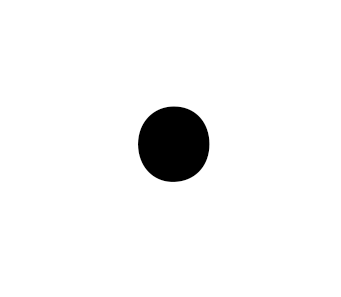
\includegraphics{fig1.png}}
% \caption{Example of a figure caption.}
% \label{fig}
% \end{figure}

% Figure Labels: Use 8 point Times New Roman for Figure labels. Use words 
% rather than symbols or abbreviations when writing Figure axis labels to 
% avoid confusing the reader. As an example, write the quantity 
% ``Magnetization'', or ``Magnetization, M'', not just ``M''. If including 
% units in the label, present them within parentheses. Do not label axes only 
% with units. In the example, write ``Magnetization (A/m)'' or ``Magnetization 
% \{A[m(1)]\}'', not just ``A/m''. Do not label axes with a ratio of 
% quantities and units. For example, write ``Temperature (K)'', not 
% ``Temperature/K''.

\section*{Acknowledgment}

The preferred spelling of the word ``acknowledgment'' in America is without 
an ``e'' after the ``g''. Avoid the stilted expression ``one of us (R. B. 
G.) thanks $\ldots$''. Instead, try ``R. B. G. thanks$\ldots$''. Put sponsor 
acknowledgments in the unnumbered footnote on the first page.

% \section*{References}

% Please number citations consecutively within brackets \cite{b1}. The 
% sentence punctuation follows the bracket \cite{b2}. Refer simply to the reference 
% number, as in \cite{b3}---do not use ``Ref. \cite{b3}'' or ``reference \cite{b3}'' except at 
% the beginning of a sentence: ``Reference \cite{b3} was the first $\ldots$''

% Number footnotes separately in superscripts. Place the actual footnote at 
% the bottom of the column in which it was cited. Do not put footnotes in the 
% abstract or reference list. Use letters for table footnotes.

% Unless there are six authors or more give all authors' names; do not use 
% ``et al.''. Papers that have not been published, even if they have been 
% submitted for publication, should be cited as ``unpublished'' \cite{b4}. Papers 
% that have been accepted for publication should be cited as ``in press'' \cite{b5}. 
% Capitalize only the first word in a paper title, except for proper nouns and 
% element symbols.

% For papers published in translation journals, please give the English 
% citation first, followed by the original foreign-language citation \cite{b6}.

\begin{thebibliography}{00}
\bibitem{b1} G. Eason, B. Noble, and I. N. Sneddon, ``On certain integrals of Lipschitz-Hankel type involving products of Bessel functions,'' Phil. Trans. Roy. Soc. London, vol. A247, pp. 529--551, April 1955.
\bibitem{b2} J. Clerk Maxwell, A Treatise on Electricity and Magnetism, 3rd ed., vol. 2. Oxford: Clarendon, 1892, pp.68--73.
\bibitem{b3} I. S. Jacobs and C. P. Bean, ``Fine particles, thin films and exchange anisotropy,'' in Magnetism, vol. III, G. T. Rado and H. Suhl, Eds. New York: Academic, 1963, pp. 271--350.
\bibitem{b4} K. Elissa, ``Title of paper if known,'' unpublished.
\bibitem{b5} R. Nicole, ``Title of paper with only first word capitalized,'' J. Name Stand. Abbrev., in press.
\bibitem{b6} Y. Yorozu, M. Hirano, K. Oka, and Y. Tagawa, ``Electron spectroscopy studies on magneto-optical media and plastic substrate interface,'' IEEE Transl. J. Magn. Japan, vol. 2, pp. 740--741, August 1987 [Digests 9th Annual Conf. Magnetics Japan, p. 301, 1982].
\bibitem{b7} M. Young, The Technical Writer's Handbook. Mill Valley, CA: University Science, 1989.
\end{thebibliography}
\vspace{12pt}
\color{red}
IEEE conference templates contain guidance text for composing and formatting conference papers. Please ensure that all template text is removed from your conference paper prior to submission to the conference. Failure to remove the template text from your paper may result in your paper not being published.

\end{document}
